% all fire columns were dropped and we kept generated a binary column indicating the presence of fire.
% since all represented fire = 1 resampling was necessary to generate non fire rows
% To prevent data leakage and ensure robust model evaluation, we first split the dataset into training and testing sets before applying resampling techniques.
\subsection{Splitting to training test and validation set}
The dataset was divided into three disjoint sets to ensure robust model evaluation and prevent data leakage. First, the target variable (fire) was separated from the features, and a stratified 70-30 split was applied to create a training set (70\%) and a temporary set (30\%). Subsequently, the temporary set was further divided equally into validation (15\%) and test sets (15\%) using the same stratification strategy. This approach ensures that each set maintains the original class distribution, which is particularly important given the class imbalance present in the wildfire data.

\subsection{Resampling Strategy for Class Imbalance}\label{subsec:resampling}

\subsubsection{Motivation: Class Imbalance in Wildfire Prediction}

The wildfire occurrence variable exhibits a strong class imbalance, with non-fire observations largely dominating fire events. This imbalance is typical in environmental risk modeling and can severely bias supervised learning algorithms toward the majority class, resulting in poor detection of rare but critical events such as wildfires \cite{he_imbalanced, japkowicz2002class}.

To address this issue, several resampling techniques were applied \emph{exclusively to the training set}. Validation and test sets were intentionally left unchanged in order to preserve an unbiased evaluation of model generalization. The objective of resampling is to improve the model’s sensitivity to fire occurrences while maintaining meaningful decision boundaries.

Figure~\ref{fig:resampling_comparison} summarizes the class distributions obtained using the different resampling strategies.

\subsubsection{Synthetic Minority Over-sampling Technique (SMOTE)}

SMOTE (Synthetic Minority Over-sampling Technique) is an over-sampling approach that generates new synthetic samples for the minority class instead of simply duplicating existing observations \cite{chawla_smote}. For each minority instance, synthetic points are created by interpolating between the sample and its $k$ nearest minority neighbors in feature space.

This method increases the representation of the minority class while preserving the underlying data structure, thereby reducing overfitting risks associated with naive duplication. In this study, SMOTE was applied with $k=5$ nearest neighbors, resulting in a perfectly balanced training set where fire and non-fire classes contain an equal number of samples.

SMOTE is particularly useful when the minority class is under-represented but sufficiently dense to allow meaningful interpolation.

\subsubsection{Tomek Links Under-sampling}

Tomek Links is an under-sampling technique designed to clean ambiguous samples near class boundaries \cite{tomek1976two}. A Tomek link is defined as a pair of samples from opposite classes that are mutual nearest neighbors. Such pairs typically lie in overlapping regions and may correspond to noisy or borderline observations.

When Tomek Links are removed, the majority-class samples involved in these pairs are eliminated, resulting in a cleaner and more separable dataset. In contrast to SMOTE, Tomek Links does not balance the dataset but slightly reduces class overlap while preserving the original class ratio.

In this work, Tomek Links was used to evaluate whether boundary cleaning alone could improve class separability without altering the overall imbalance structure.

\subsubsection{Combined SMOTE + Tomek Links}

The SMOTE+Tomek strategy combines the strengths of both over-sampling and under-sampling \cite{batista2004study}. First, SMOTE is applied to generate synthetic minority samples and balance the dataset. Then, Tomek Links are identified and removed to clean overlapping regions created during the over-sampling process.

This hybrid approach aims to achieve both class balance and improved class separation. In the context of wildfire prediction, this method provides a more robust training set by increasing minority representation while simultaneously reducing noise near decision boundaries.

As shown in Figure~\ref{fig:resampling_comparison}, SMOTE+Tomek yields a balanced dataset similar to SMOTE, but with slightly fewer samples due to the removal of ambiguous points.

\subsubsection{Comparison and Practical Considerations}

The resampling strategies serve different purposes:
\begin{itemize}
  \item \textbf{Original}: Preserves the true data distribution but strongly favors the majority class.
  \item \textbf{SMOTE}: Balances classes through synthetic generation, improving recall of fire events.
  \item \textbf{Tomek Links}: Cleans class boundaries without enforcing balance.
  \item \textbf{SMOTE+Tomek}: Balances the dataset while reducing class overlap, often yielding more stable classifiers.
\end{itemize}

For subsequent modeling experiments, all four versions of the training data were retained to allow a systematic comparison of model sensitivity to resampling choices.

\begin{figure}[H]
  \centering
  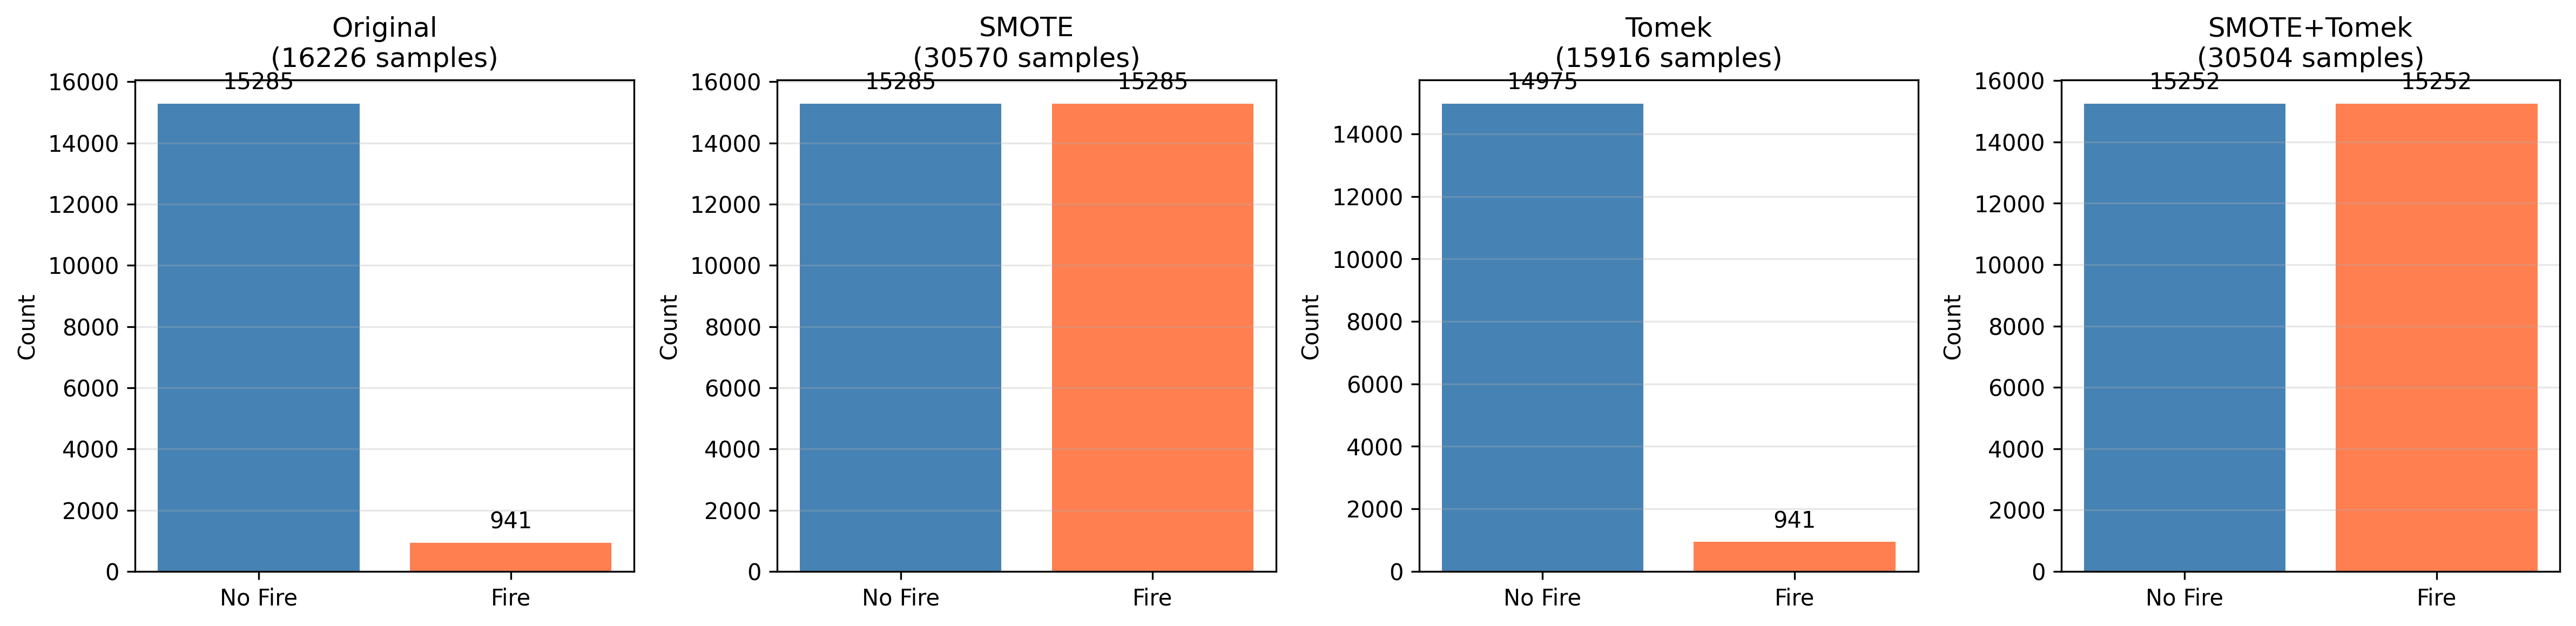
\includegraphics[width=0.98\linewidth]{images/MergedPreprocess/resampling_comparison.png}
  \caption{Comparison of class distributions in the training set before and after resampling. From left to right: original distribution, SMOTE over-sampling, Tomek Links under-sampling, and combined SMOTE+Tomek.}\label{fig:resampling_comparison}
\end{figure}

